\section{Extruder}

An extruder end-effector was designed and fabricated for the carbon fiber 3D printer. The extruder is the mechanism responsible for depositing the filament in a 3D printing system. Generally, this mechanism includes a motor that drives a gripping mechanism, which reels in and pushes the filament into a nozzle. A heating element just prior the the nozzle melts the outside of the plastic filament while softening the interior. The molten filament is extruded through the nozzle outlet onto the printing bed or an already existing printed layer where it cools to create the part.\\

In the case of the curved layer carbon fiber 3D printer, the extruder was required to mount to the FANUC robot arm, be compact\footnote{The compact size is required for two reasons. First, to ensure that induced torque on the robot arm joints and gripper remain within safe operating conditions. Second, to readily permit the nozzle to deposit material when not perpendicular to the build platform, which will be required for printing curved layers.}, and accept filaments of a variety of sizes (likely ranging in diameter from 1.75 mm to 3 mm). \\

\subsection{Design}

\indent

Figure~\ref{fig:old extruder} presents the initial design of the extruder in \emph{SolidWorks}. This iteration of the extruder design mounted to the Fanuc grippers and was intended to be made from custom-machined components (acrylic and aluminum) and RepRap hardware (nozzle, J-head, J-head mounting plate, ceramic heating element, thermistor, fan, and fan mount). This configuration locates the nozzle outlet along the mid-plane of the grippers for simple coordinate transformations when programming the robot to print. Laser-cut acrylic gears provide a 3:1 step up in torque from the stepper motor and drive a notched screw, which grips and pushes the filament into the nozzle. A bearing opposite the screw provides counter-pressure and its mounting plates can adjust the distance between the screw and bearing to accommodate different filament sizes.\\

\begin{figure}[h!]
\centering
\includegraphics[width=0.5\textwidth]{./figures/extruder-old-2}
\caption{An isometric view of the initial extruder design.}
\label{fig:old extruder}
\end{figure}

To assess the feasibility of the initial extruder design, minor tweaks were implemented within the CAD to make a laser-cut prototype.  Figure~\ref{fig:prototype extruder} shows the prototype mounted on the FANUC grippers. The prototype served its purpose and demonstrated numerous problems with the initial design. There were some mis-measurements of RepRap hardware, using spacers instead of threaded standoffs decreased the rigidity of the structure, the structure was a bit larger than desired, and a few undetected interferences were discovered. Subsequently, the extruder went through a redesign phase to develop an acceptable configuration.\\

\begin{figure}[h!]
\centering
\includegraphics[width=0.5\textwidth]{./figures/extruder-prototype-2}
\caption{A photograph of the mounted prototype.}
\label{fig:prototype extruder}
\end{figure}

Figure~\ref{fig:extruder iso} presents a rendering of the final extruder design. Figure~\ref{fig:extruder drawing} provides general dimensions and annotations to fully present the extruder design concept. The final design was significantly smaller than the initial design, requird less machining, and used less fastening hardware. The size decrease was accomplished by using smaller gears (50\% scaled versions of gears dimensions taken from \emph{SDP-SI}\footnote{\url{http://www.sdp-si.com/}} and located the stepper motor directly beneath the FANUC grippers. As part of the design process the gears were laser-cut, and physically tested to ensure that the teeth would not shear off under a load less than the stall torque of the stepper motor, before being fully committed to this design. The stepper motor (Sparkfun ROB-10846) outputs 68 oz-in of torque and has a resolution of 400 steps/revolution. Two laser-cut acrylic gears step up the torque to 204 oz-in.\footnote{Most extruders in the 3D printing community use analogous stepper motors and utilize gear trains to step up the torque. Common gear ratios range from 2:1 to 4:1 depending on the specific qualities of the filament. Given that the specifics of the filament are not yet fully determined, the mean value was used.} In this design, a partially threaded screw is would be notched on the mill to contain teeth-like features along a portion of its length. These teeth will grip the filament and push it into the extruder.\footnote{Concerns were raised that six teeth-like features may not be enough to sufficiently grip the filament. However, without a finalized filament at the time to test with, the design moved forward under the assumption that a dremel could be used to manually carve in more indents in the future if necessary.} The screw rides along two bronze PTFE-coated bearings to ensure smooth rotation during printing. Two adjustment plates locate a bearing just opposite the screw to provide counter-pressure during printing. The plates are secured in place using four screws, which can be loosened or tightened to adjust the distance between the screw and bearing to accommodate different filament sizes. Shims or spring washers may have to be utilized to located this adjustable mechanism in its optimal position for the official CFRP. The entire extruder assembly secures to the FANUC gripper with four screws.\\

This extruder design requires custom machined aluminum pieces. Many 3D printers utilize 3D printed bodies for mounting RepRap hardware, but the associated poor tolerances and material flexibility are not ideal for the curved layer carbon fiber 3D printer. Additionally, it was believed that aluminum would allow for simple machining modiciations if any future adjustments are necessary after manufacturing and testing.\\

\begin{figure}[h!]
\centering
\includegraphics[width=0.5\textwidth]{./figures/extruder-iso}
\caption{An isometric render of the final extruder design.}
\label{fig:extruder iso}
\end{figure}

\begin{figure}[h!]
\centering
\includegraphics[width=1\textwidth]{./figures/extruder-drawing}
\caption{A general drawing of the final extruder design.}
\label{fig:extruder drawing}
\end{figure}

\clearpage

\subsection{Fabrication}

\indent

The extruder's custom-machined aluminum components were fabricated in Cooper Union's Student Machine Shop. The \emph{SolidWorks} drawings used for manufacturing the extruder are located in the appendix. All pieces were roughly cut to size on the band saw and then squared up to outer dimensions on the 3-axis mill using endmill bits. Holes were creating using the endmills, drill bits, and boring bars depending on the type of fit and dimension. Most pieces required multiple setup to fabricate all features. Threaded holes were tapped while pieces were still set up in the mill to ensure vertical tapping perpendicular to the face.\footnote{Aluminum is a relatively soft metal. Without a setup to maintain proper tap alignment, such as tapping freely by hand, it is very easy for the tap to thread the hole at a few degrees off of the vertical. For short screws, extending only one or two times the nominal diameter of the screw this effect is not very visible. For long screws, such as a 1 1/4 inch 4-40, this effect could break and entire design and require the piece to be remade.}\\

\subsubsection{Progress Photos}

%squaring

\indent

Figure~\ref{fig:extruder-progress-square} through Figure~\ref{fig:extruder-progress-4} show photos of the extruder assembly's progress through the weeks of fabrication. Figure~\ref{fig:extruder-mistake-1} and Figure~\ref{fig:extruder-mistake-2} show photos of two major machining mistakes made during the fabrication process. Due to the severity of these two mistakes extra time was spent remaking these pieces. All other minor errors were easily rectified, such as accidentally swapping which hole was a threaded or thru-hole for clamping two plates together.\\

\begin{figure}[h!]
\centering
\includegraphics[width=0.5\textwidth]{./figures/extruder-progress-square}
\caption{Extruder machining progress photo: some square up pieces.}
\label{fig:extruder-progress-square}
\end{figure}

%progress

\begin{figure}[h!]
\centering
\includegraphics[width=0.5\textwidth]{./figures/extruder-progress-1}
\caption{Extruder machining progress photo: Staring the main assembly. Stepper shaft complete.}
\label{fig:extruder-progress-1}
\end{figure}

\begin{figure}[h!]
\centering
\includegraphics[width=0.5\textwidth]{./figures/extruder-progress-2}
\caption{Extruder machining progress photo: A closeup of the first two completed pieces.}
\label{fig:extruder-progress-2}
\end{figure}

\begin{figure}[h!]
\centering
\includegraphics[width=0.5\textwidth]{./figures/extruder-progress-3}
\caption{Extruder machining progress photo: One view of the bearing holders and J-head mount fully assembled.}
\label{fig:extruder-progress-3}
\end{figure}

\begin{figure}[h!]
\centering
\includegraphics[width=0.5\textwidth]{./figures/extruder-progress-4}
\caption{Extruder machining progress photo: Another view of the bearing holders and J-head mount fully assembled.}
\label{fig:extruder-progress-4}
\end{figure}

%machining error

\begin{figure}[h!]
\centering
\includegraphics[width=0.5\textwidth]{./figures/extruder-mistake-1}
\caption{Extruder machining progress (and error) photo: One of the adjustment plates with a squaring error.}
\label{fig:extruder-mistake-1}
\end{figure}

\begin{figure}[h!]
\centering
\includegraphics[width=0.5\textwidth]{./figures/extruder-mistake-2}
\caption{Extruder machining progress (and error) photo: One of the adjustment plates with a concentricity error with an otherwise nearly complete extruder.}
\label{fig:extruder-mistake-2}
\end{figure}

\clearpage

\subsubsection{Machining Photos}

% photos from the machine shop

\indent

Figure~\ref{fig:extruder-edge-finder} through Figure~\ref{fig:extruder-screw-mill} are photos of machining processes being performed on extruder parts while in the shop. Notice how all the images are of pieces on the mill. Except for putting a flat on the stepper motor shaft (rough cut with a dremel and filed to size) and laser cuttig acrylic gears, all custom components were fabricated with the mill.\\

\begin{figure}[h!]
\centering
\includegraphics[width=0.5\textwidth]{./figures/extruder-edge-finder}
\caption{Extruder machining in action: Indicating a part with an edge-finder}
\label{fig:extruder-edge-finder}
\end{figure}

\begin{figure}[h!]
\centering
\includegraphics[width=0.5\textwidth]{./figures/extruder-tap}
\caption{Extruder machining in action: Tapping on the mill.}
\label{fig:extruder-tap}
\end{figure}

\begin{figure}[h!]
\centering
\includegraphics[width=0.5\textwidth]{./figures/extruder-screw-mill}
\caption{Extruder machining in action: Notching the screw with a 1/16 inch endmill.}
\label{fig:extruder-screw-mill}
\end{figure}

\clearpage

\subsubsection{Assembly Photos}

% assembly photos

\indent

Figure~\ref{fig:extruder-first-mount} through Figure~\ref{fig:extruder-mechanism} are photos of the mounted extruder assembly. Figure~\ref{fig:extruder-first-mount} shows the very first attempt of assembling the extruder to the gripper on the FANUC robot. Notice how the laser-cut gears are not present in this assembly since they were not yet cut. Managing the wires during the assembly proved to be a little challening but ultimately did not require the implementation of a disconnect mechanism on the wires (ie. molex connectors). Figure~\ref{fig:extruder-mounting} highlights some of the gripper mounting features which are not easily seen from a side view and invisible from the front. The gripper jaws contain metric sized holes, through which screws were inserted and threaded into the extruder assembly for additional stability (there are threaded metric screw holes on the upper front of the gripper module which are also utilized as connection points). Figure~\ref{fig:extruder-side-profile} shows the extruder from the side while printing ABS. In addition to highlighting main mechanism (gears and notched screw), this profile also shows kapton tape (translucent, heat resistant tape) that is used to fix wires to the extruder assembly. Finally, Figure~\ref{fig:extruder-mechanism} is a close-up of the extruder mechanism. As intended, the filament is actuated by a notched screw and is held in place by a bearing with adjustable distance. The adjustments plates utilize lockwashers, which act as springs, between the main assembly to statically hold the bearing in multiple positions that accomadate different filament widths.\\

\begin{figure}[h!]
\centering
\includegraphics[width=0.5\textwidth]{./figures/extruder-first-mount}
\caption{The first (and seemless) attempt of mounting the fabricated extruder to the FANUC gripper.}
\label{fig:extruder-first-mount}
\end{figure}

\begin{figure}[h!]
\centering
\includegraphics[width=0.5\textwidth]{./figures/extruder-mounting}
\caption{A close-up of the fabricated extruder's gripper mounting fixtures.}
\label{fig:extruder-mounting}
\end{figure}

\begin{figure}[h!]
\centering
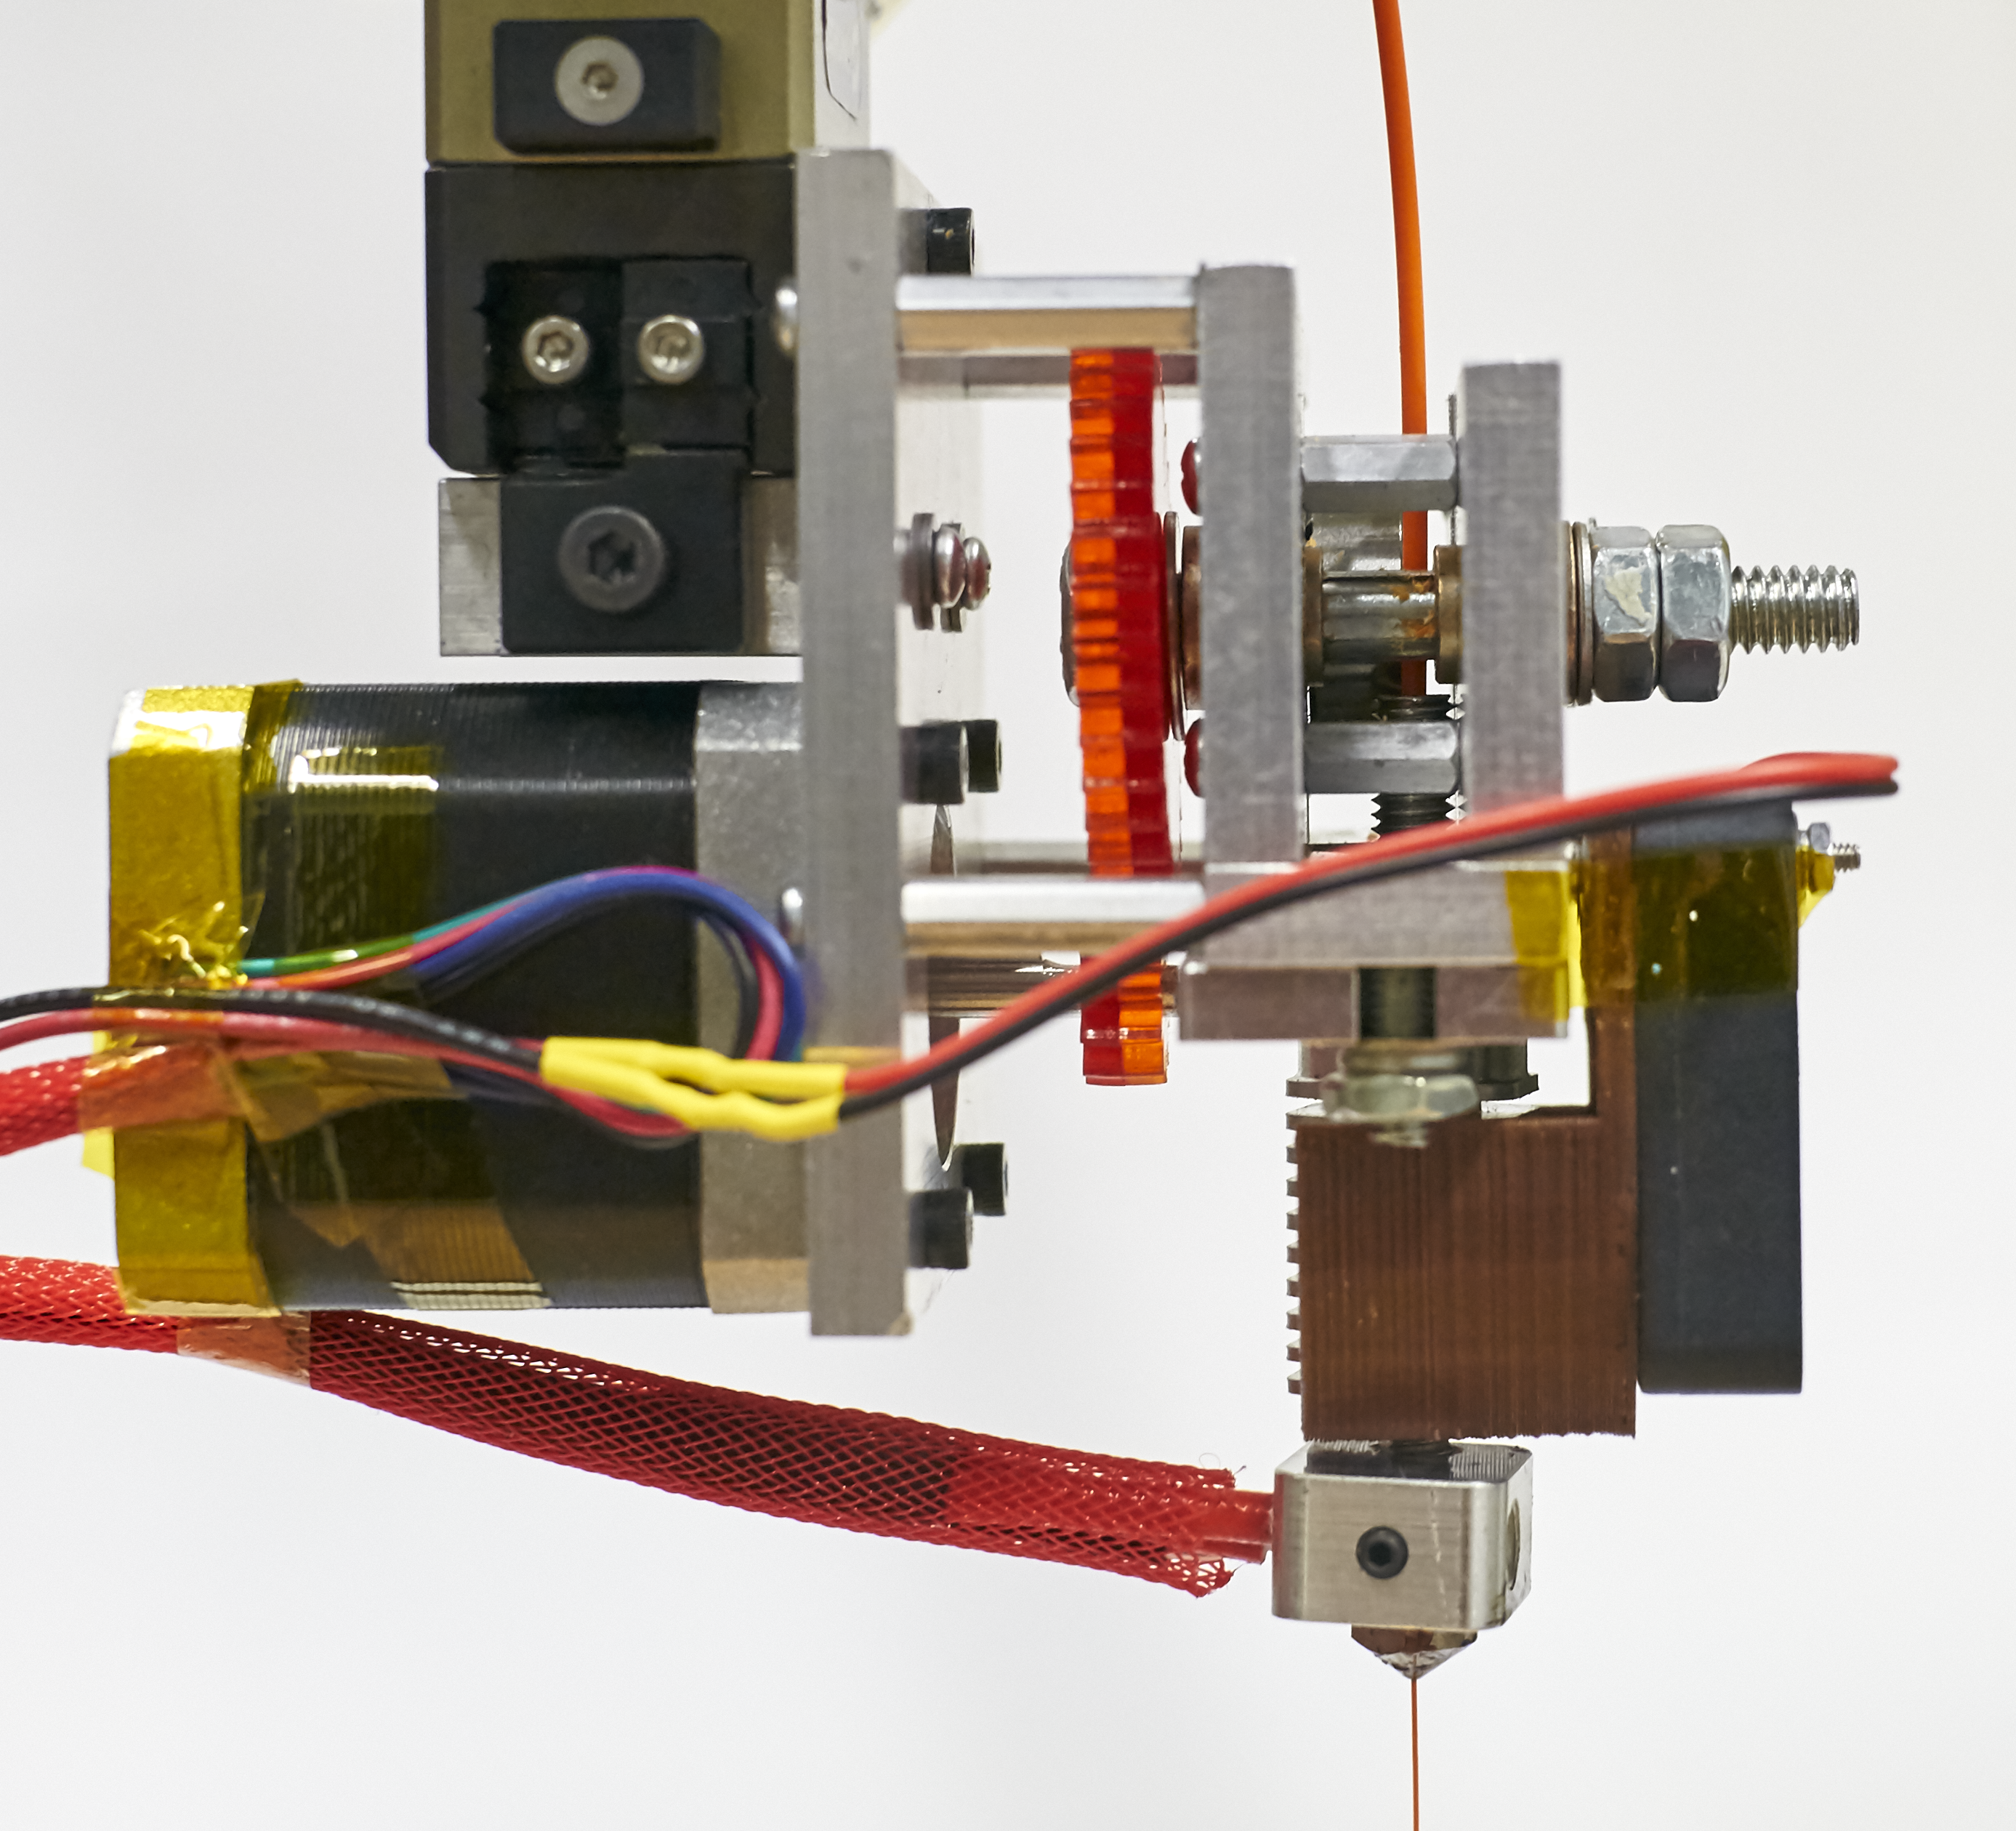
\includegraphics[width=0.5\textwidth]{./figures/extruder-side-profile}
\caption{A side view of the fabricated (and extruding) extruder.}
\label{fig:extruder-side-profile}
\end{figure}

\begin{figure}[h!]
\centering
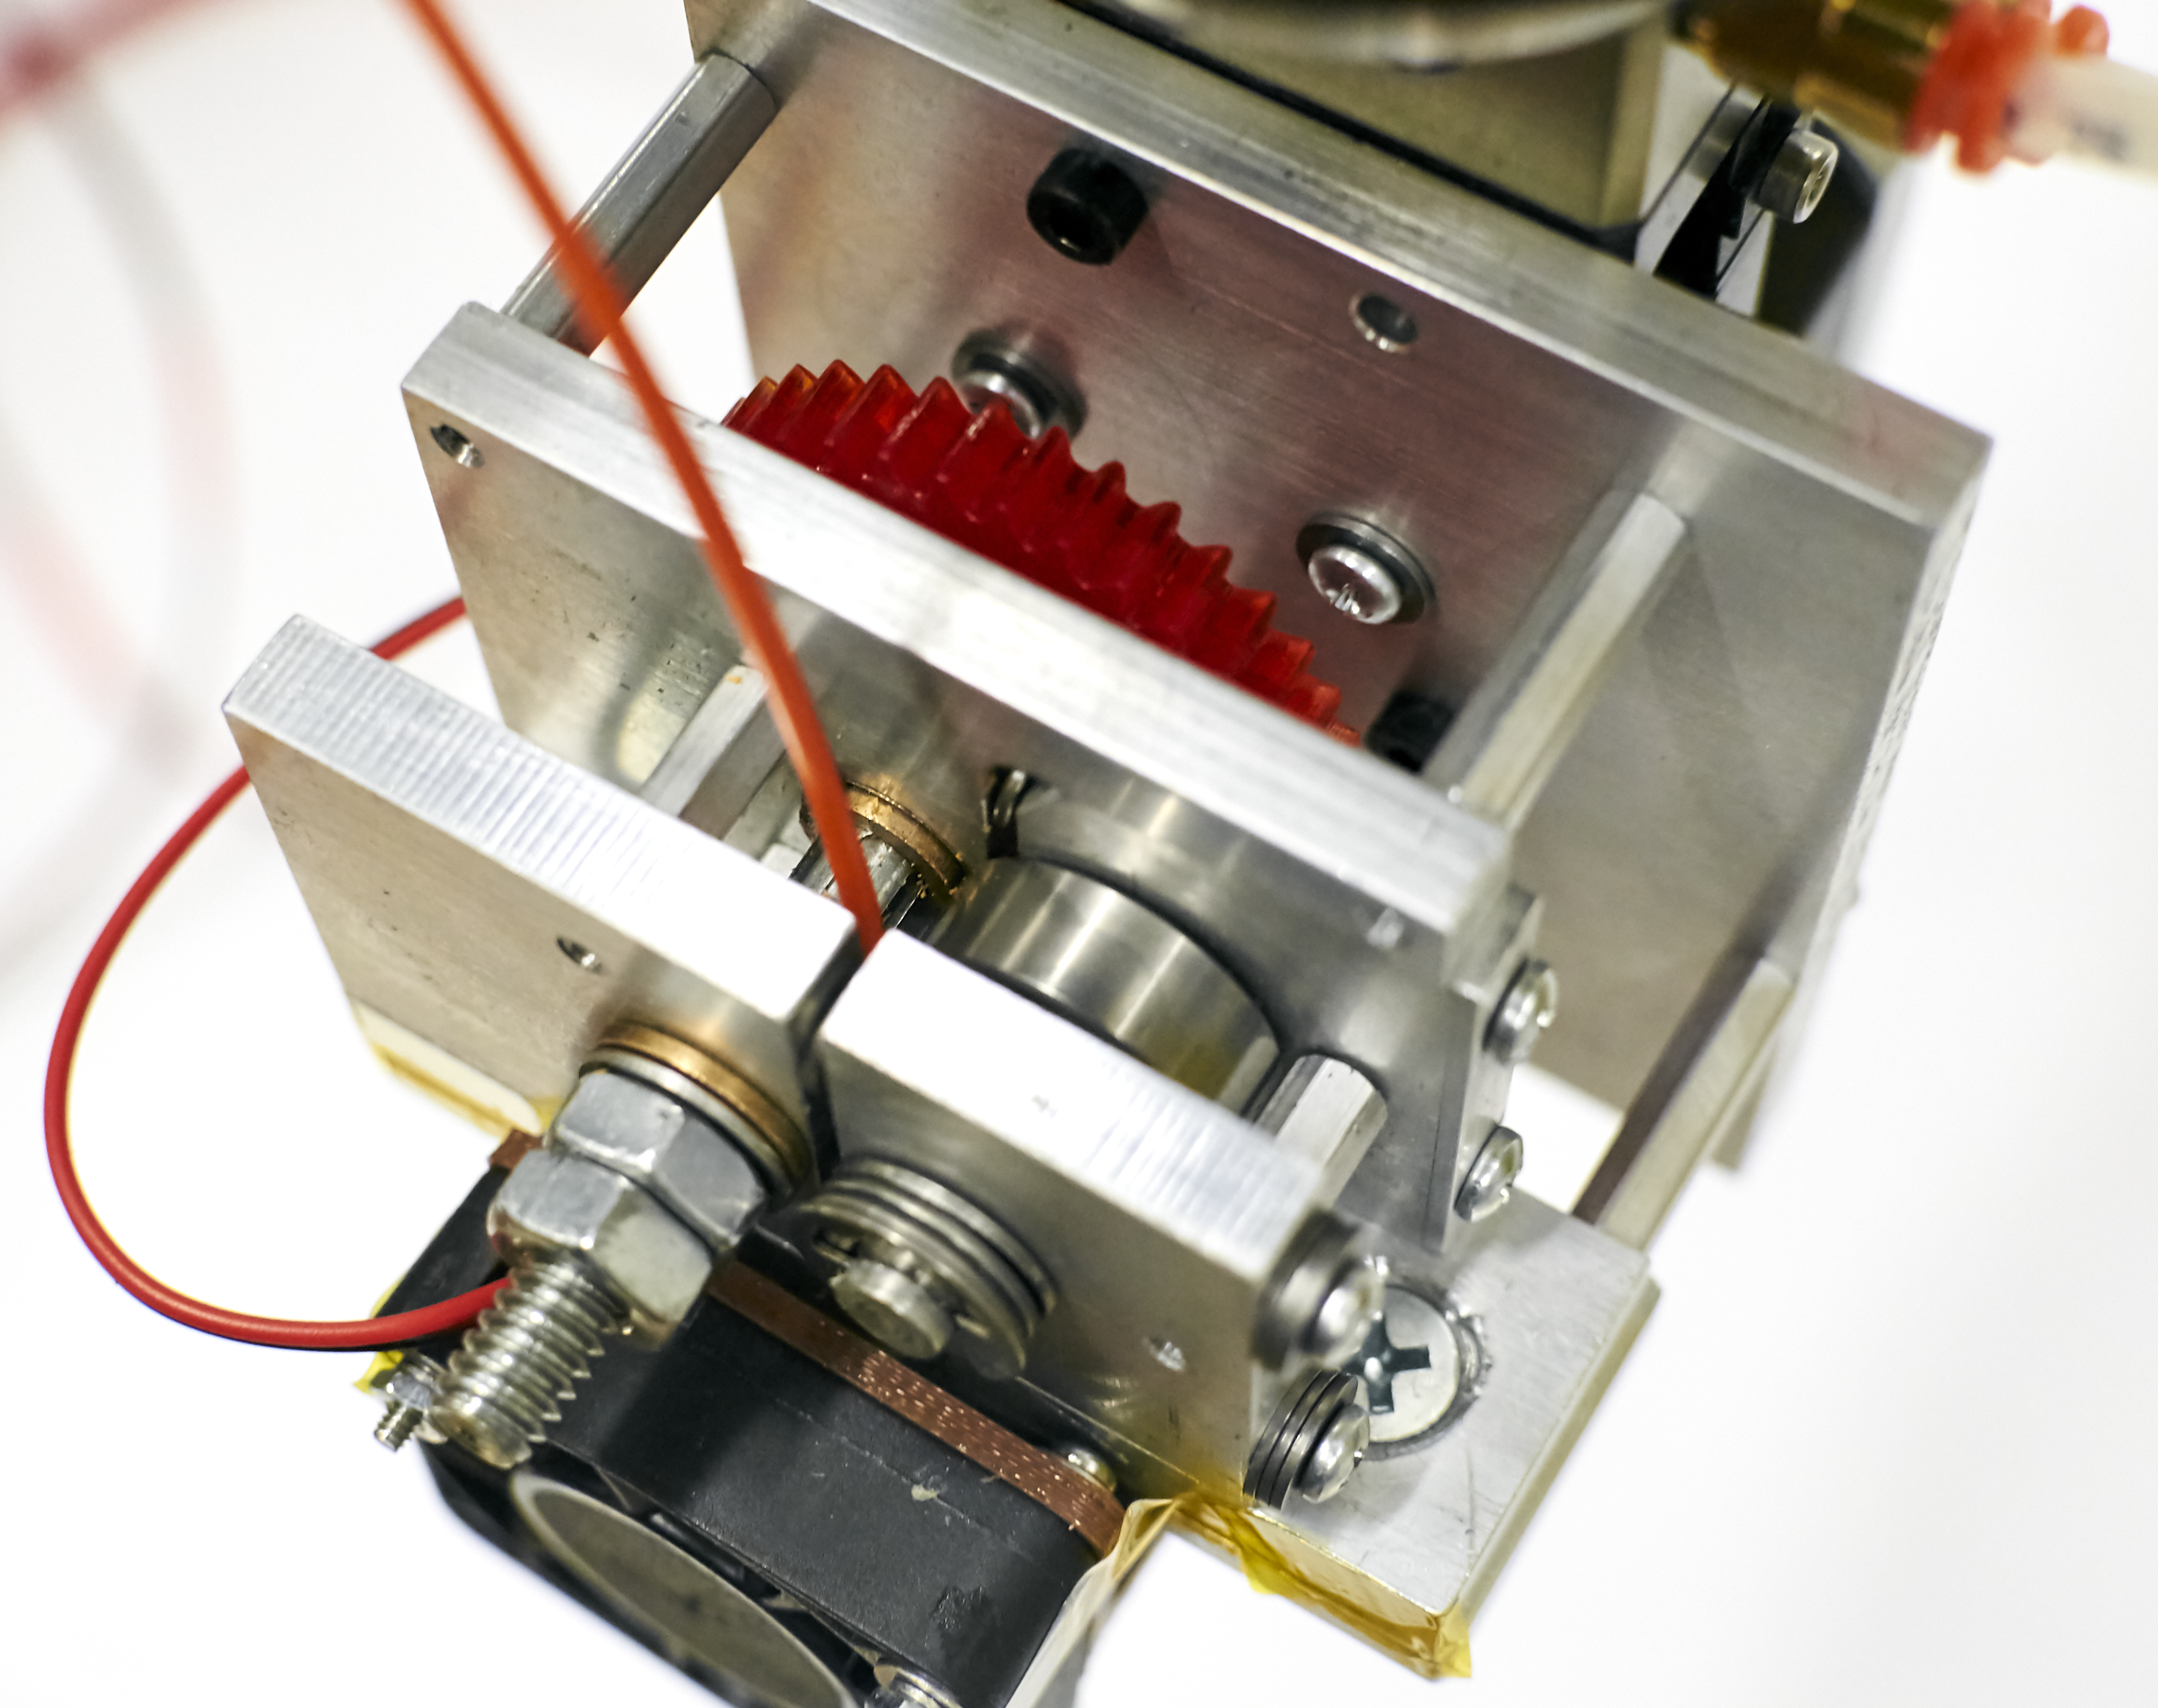
\includegraphics[width=0.5\textwidth]{./figures/extruder-mechanism}
\caption{A close-up view of the fabricated extruder's main mechanism.}
\label{fig:extruder-mechanism}
\end{figure}

\clearpage

\subsection{Implementation}

\indent

After assembling the extruder on the FANUC robot its functionality was tested using 1.75 mm ABS filament from MakerBot. Figure~\ref{fig:extruder-edge-finder} shows an image of this test. The extruder was able to print the ABS, meaning that the extruder was designed and built properly (the notched screw provided enough traction on the filament, the bearing provided adequate counterpressure, the adjustment plates we compliant to the filament size, the stepper motor and gears were aligned properly and provided enough driving torque, and the heater reached the neceesary temperature).\footnote{At the time that this paper is being written, the CFRP filament has not yet been tested on the extruder. Given that the CFRP filament will be the same diameter and the gripping depth of the screw will only interact with solid ABS, the extruder's performance is not expected to differ.}\\

\begin{figure}[h!]
\centering
\includegraphics[width=0.5\textwidth]{./figures/extruder-abs-extrude}
\caption{The fabricated extruder successfully pulling in ABS filament and printing through the nozzle.}
\label{fig:extruder-abs-extrude}
\end{figure}
